
  \section{Results}
  
  In this section the results for the US Airline Passenger Dataset are
  presented. First, the model specifications and results of graph
  representation learning and GNNs are presented. Afterwards, the graph machine
  learning results are compared to the results of "standard" machine
  learning methods.

  \subsection{Graph Representation Learning}

  The training graph consisting of 6'000 nodes which is a sub-sample of the
  US Airline Passenger training dataset provided on Kaggle \citep{KAGGLE2015}.
  2 Dimensional node representations were learned using the Node2Vec algorithm
  \citep{grover2016node2vec}. The model settings were defined as follows:

  \begin{itemize}[itemsep=1mm]
    \item Dimensions: 2
    \item Random walk length: 8
    \item Number of random walks: 100
    \item Window size: 10
    \item Node batch size: 2
    \item Return parameter $p=1$
    \item In-out parameter $q=1$
  \end{itemize}

  \noindent With the specified Return- and In-out parameter, the Node2Vec
  output corresponds to the DeepWalk output. The resulting node embeddings were
  then used as inputs for standard machine learning methods. An overview of the
  node embeddings is shown in figure \ref{fig:node2vec}. 

  \begin{figure}[h]
		\centering
		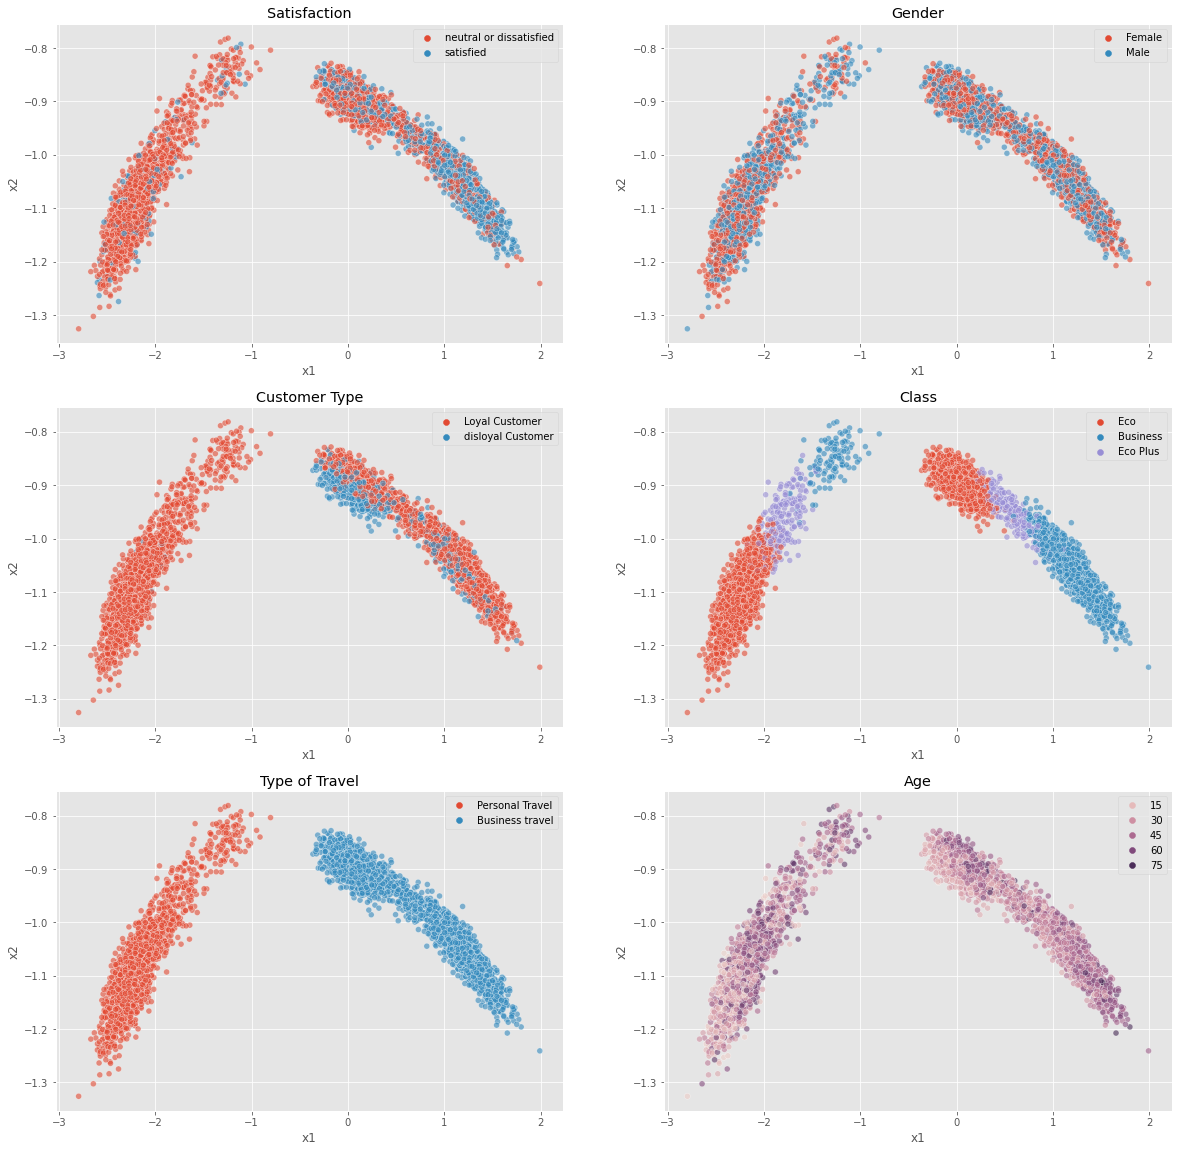
\includegraphics[width=0.7\textwidth]{node2vec_emb.png}
		\caption{Node2Vec embeddings}
        \label{fig:node2vec}
  \end{figure}

  \noindent The embeddings reveal very interesting insights in term of cluster
  analysis. First, the observation seen in figure \ref{fig:us_airline_graph}
  mainly correspond to the observations in figure \ref{fig:node2vec}. The
  advantage of graph representation learning, is that the nodes plotted using
  Node2Vec corresponds to a proper scatter plot in Euclidean space. In
  addition, the nodes are group in a much nicer and more orderly fashion. This
  makes it possible to infer with a higher level of certainty that for instance
  business class passengers traveling for business purposes tend to be more
  satisfied than other passengers on average. The 2 dimensional node embeddings
  thus provide interesting insights for cluster analysis. \\

  \noindent The node embeddings were used for three standard machine learning
  methods which are presented in table \ref{table:node2vec_results}.

  \begin{table}[h]
    \centering
    \begin{tabular}{|l||l|l|}
      \hline
      \textbf{ML Method} & \textbf{Training Accuracy} & \textbf{Validation
      Accuracy}\\
      \hline\hline
      Logistic Regression & 76.85\% & 75.83\% \\\hline 
      Support Vector Machine & 76.95\% & 75.66\% \\\hline
      ANN & 77.61\% & 76.58\% \\
      \hline
    \end{tabular}
    \caption{Node2Vec Classification Results}
    \label{table:node2vec_results}
  \end{table}

  \noindent The results show, that Node2Vec only has very modest success in
  classifying passengers according to their satisfaction. When looking at the
  satisfaction scatter plot in figure \ref{fig:node2vec} it becomes obvious why
  the downstream machine learning tasks only had limited success. For the
  variables which were used for generating the graph and for which neighborhood
  clusters emerged, Node2Vec created very good node embeddings. The label
  variable satisfaction could not be used for the graph generation as this would
  be unrealistic. Since the label is not considered for the graph generation,
  Node2Vec does not create embeddings which consider the label. The label is
  only considered to the extend that the variables used for the graph
  generation process create structures which are related somehow to the label.
  For that reason, the success of any downstream machine learning method will
  be limited to the extent that the node labels capture relevant information
  for predicting the label. 

